\setcounter{chapter}{-1}
\chapter{Introduction}

In December 2003, the idea for a new fictional language was born, an idea that 
turned out to stick with me for over 10 years now.\footnote{A lot of the text 
here is taken from the blog article, ``\citetitle{benung:happybirthday}'' 
\parencite{benung:happybirthday}.} At that time, my seventeen years old self 
was still fairly new to this whole making-up languages business, read things 
about linguistics here and there, and was not shy to ask questions about 
terminology (and, looking at old mails, a little impertinently teenager-like 
so), for example on \tit{Conlang-L} and the \tit{Zompist Bulletin Board}. One 
thing seemed to catch my interest especially: syntactic alignments other than 
the \Nom{}/\Acc{} of the few languages I was familiar with, that is, German, 
English, and French. Apparently this curiosity was big enough for me to grow 
bored with my second fictional language, Daléian (declared `quite complete' 
after maybe half a year of work or so), and to start something new from scratch 
in order to put newly acquired knowledge to test.

I had read about `trigger languages' on \tit{Conlang-L} and wanted to try my 
hands on making my own. I cannot remember how long it took me to come up with a 
first draft of an Ayeri grammar, however, I do remember having been told that a 
good language cannot be made in a summer. Of course, I still did not really 
know what I was doing then, even though I thought I had understood things and 
authoritatively declared ``this is how it works'' in my first grammar draft 
when things sometimes really do not work that way. But at least an interest had 
been whetted.

In order to illustrate the various stages from the beginnings to current Ayeri,
I went through some old backups contemporary with the very early days. 
Here is a sentence from the oldest existing document related to it, titled 
``Draft of \& Ideas for my 3rd Conlang'' -- the file's last-changed date is 
\DTMdate{2003-12-14}, though I remember having started work on Ayeri in early 
December. I added glossing for convenience and according to what I could 
reconstruct from the notes. This uses vocabulary and grammatical markers just 
made up on the spot and for illustrative purposes; little of it actually 
managed to make it into actual work on Ayeri:

\ex\begingl
	\gla Ayevhoi agiaemaesim coyaielieðamavir vhaieloyaŋaiye. //
	\glb Ay-evhoi agia-ema-esim coyai-el-i-eðam-avir vhai-el-o-yaŋa-iye //
	\glc \Tsg{}.\An{}-\Sbj{} read-\Vb{}-\Sbj{}.\An{} book-\Nn{}-\An{}-\Indf{}-\Parg{} bed-\Nn{}-\Inan{}-on-\Loc{} //
	\glft `He reads a book on the bed.' //
\endgl\xe

According to the grammar draft of \DTMdate{2004-09-05}, this would have already 
changed to:

\ex\begingl
	\gla Ang layaiyạin mecoyalei ling *pinamea. //
	\glb Ang laya-iy-a-in me-coya-lei ling *pinam-ea //
	\glc \Aarg{}.\Sbj{} read-\Tsg{}.\An{}₁-a₁-\Sbj{} \Indf{}.\Inan{}-book-\PargI{} top.of bed-\Loc{} //
	\glft `He reads a book on the bed.' //
\endgl\xe

The word \xayr{pinmF}{pinam}{bed} was only (re-)introduced on October 24, 2008. 
In the current state of Ayeri, I would translate the sentence as follows:

\ex\begingl
	\gla Ang layaya koyaley ling pinamya. //
	\glb Ang laya=ya.Ø koya-ley ling pinam-ya //
	\glc \AgtT{} read=\Tsg{}.\M{}.\Top{} book-\PargI{} top.of bed-\Loc{} //
	\glft `He reads a book on a/the bed.' //
\endgl\xe

As you can see, quite a bit of morphology got lost already early on, especially 
the overt part-of-speech marking (!) and animacy marking on nouns. Also, 
prepositions were just incorporated into a noun complex as suffixes apparently. 
Gender was originally only divided into animate and inanimate, but I changed 
that at some point because only being familiar really with European languages, 
it felt awkward to me not to be able to explicitly distinguish `he', `she', and 
`it'.

A feature that also got lost is the assignment of thematic vowels in personal 
pronouns to 3rd-person referents: originally, every 3rd-person referent newly 
introduced into discourse would be assigned one of /a e i o u/ to disambiguate, 
and there was even a morpheme to mark that the speaker wanted to dissolve the 
association. Constituent order was theoretically variable at first, but I 
preferred \textsc{svo/avp} due to familiarity with that. Later on, however, I 
settled on \textsc{vso/vap}. Also, I had no idea about what was called 
``trigger morphology'' on \tit{Conlang-L} for the longest time -- essentially, 
this referred to the Austronesian, or Philippine, aligment. I am not claiming 
that I know all about it now, just that due to reading up on the topic, I have 
a slightly more informed understanding now. Orthography changed as well over 
the years, so \orth{c} in the early examples encodes the /k/ sound, not /tʃ/ as 
it does today; diphthongs are spelled as \orth{Vi} instead of modern \orth{Vy}.

What was definitely beneficial for the development of Ayeri was the ever 
increasing amount of linguistics materials available online and my entering 
university (to study literature) in 2009, where I learned how to do research 
and also had a lot of interesting books available at the library.

One of the things people regularly compliment me on is Ayeri's script -- note, 
however, that Tahano Hikamu was not the first one I came up with for Ayeri. 
Apparently, I had already been fascinated with the look of Javanese/Balinese 
writing early on; \autoref{fig:ayeriscript2004} shows a draft dated 
\DTMdate{2004-02-09}. However, since the letter shapes in this draft looked so 
confusingly alike that I could never memorize them. About a year later, I came 
up with the draft in \autoref{fig:th2005}. What is titled ``Another 
Experimental Script'' here is what would later turn into Tahano Hikamu, Ayeri's 
`native' script. According to the notes in my fictional language ring binder, 
the script looked much the same as today about a year from then, but things 
have only been mostly stable since about 2008.

\begin{figure}
	\centering
	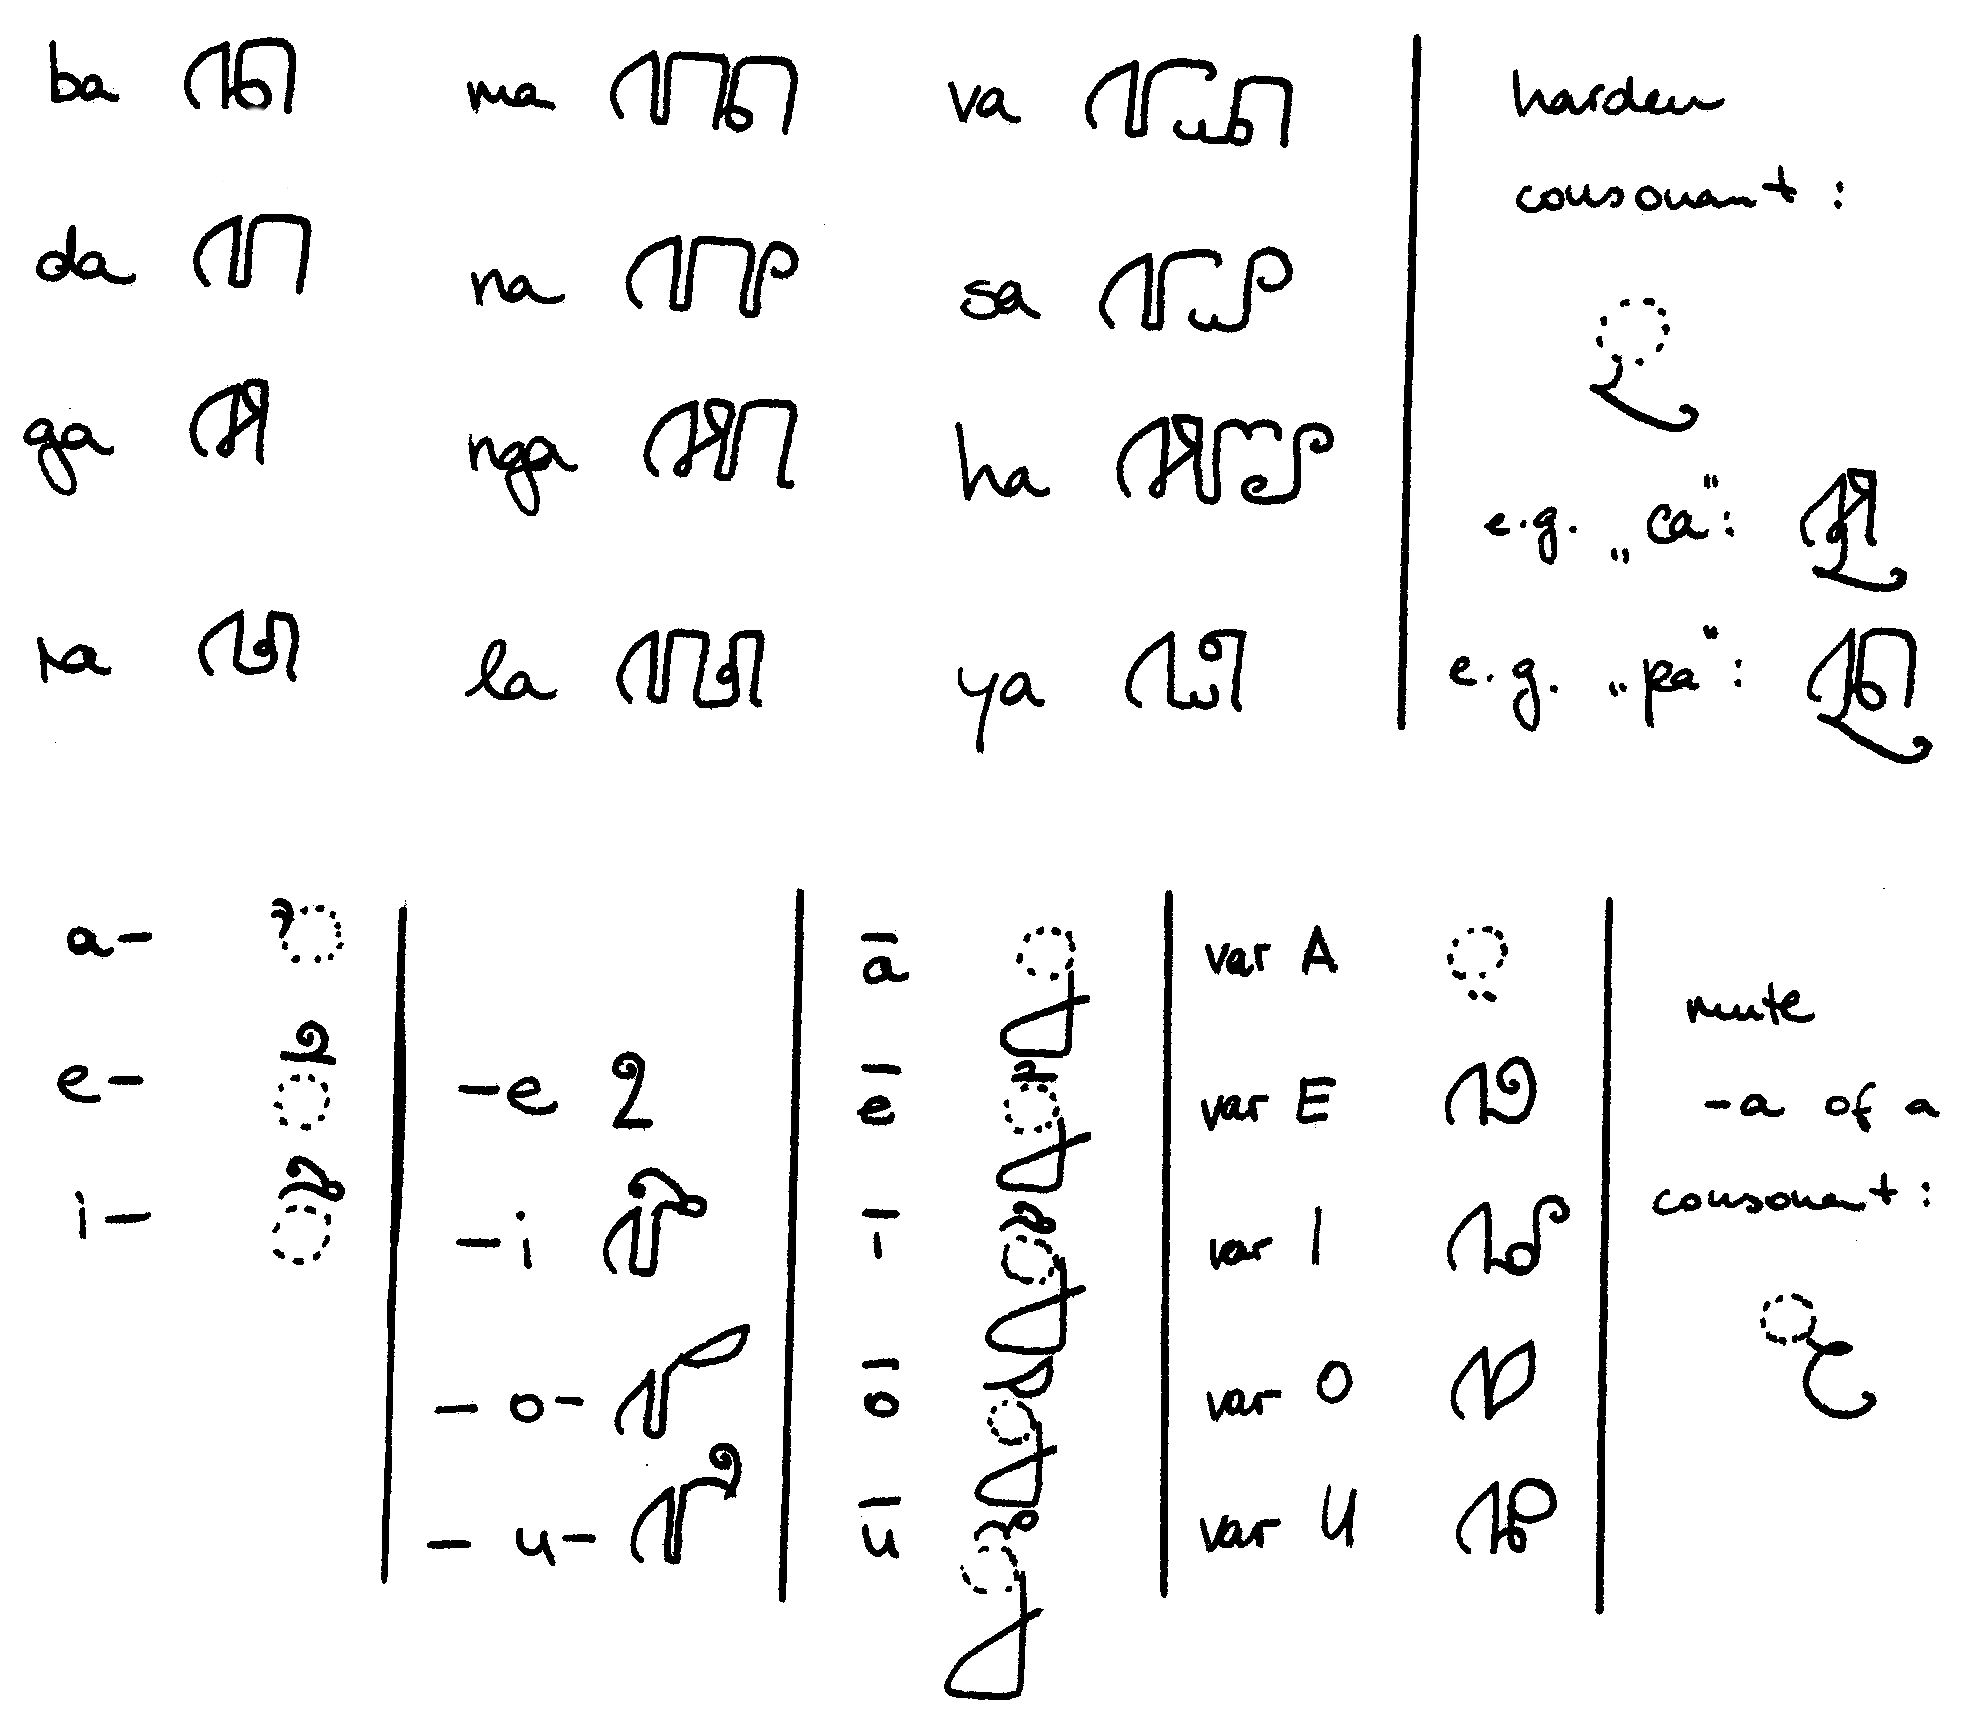
\includegraphics[width=\textwidth, keepaspectratio]{images/ayeriscript2004-300dpi-bw.png}
	\caption[First design for an Ayeri script]{First design for an Ayeri script (\DTMdate{2004-02-09})}
	\label{fig:ayeriscript2004}
\end{figure}

\begin{figure}
	\centering
	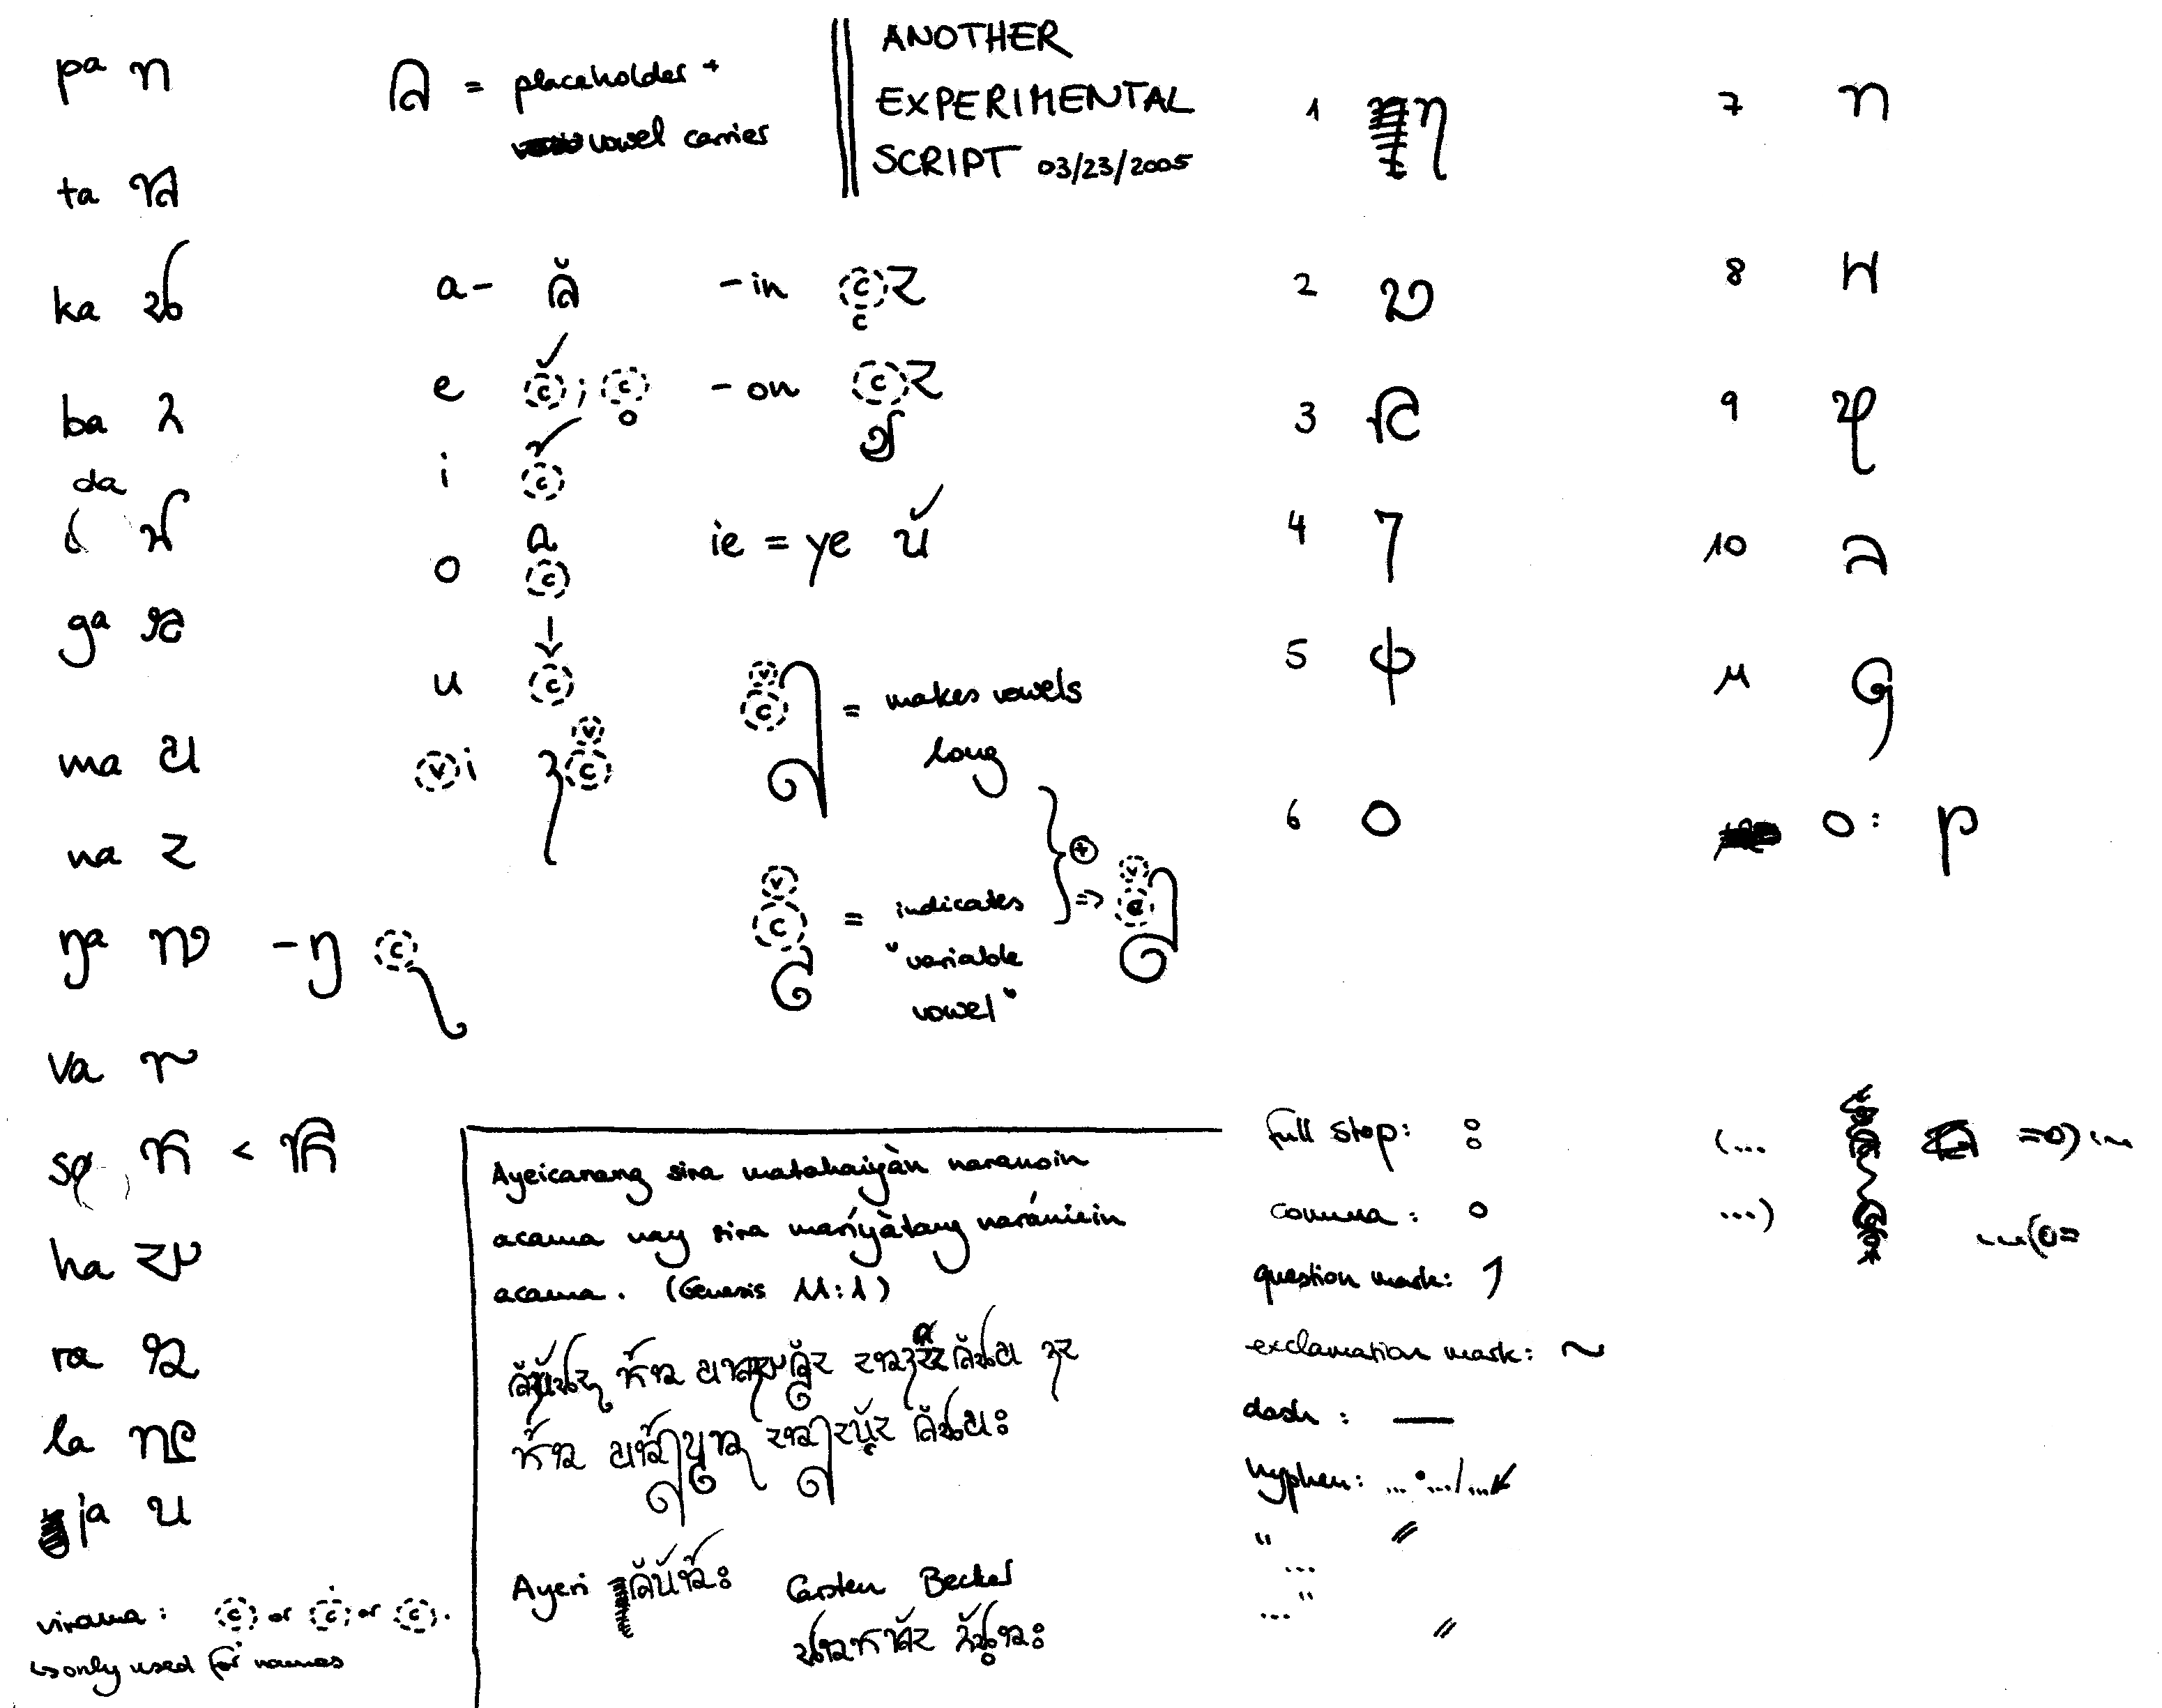
\includegraphics[width=\textwidth, keepaspectratio]{images/th2005-300dpi-bw.png}
	\caption[First draft for Tahano Hikamu]{First draft for Tahano Hikamu (\DTMdate{2005-03-23})}
	\label{fig:th2005}
\end{figure}

Another important date in the history of Ayeri is when I decided to set up an 
improved website for Ayeri that would include a blog. The idea was that this 
way, I could more freely write on whatever detail I currently worked on in 
Ayeri, outside of the constraints of the grammar. Thus, \tit{Benung.~The Ayeri 
Language Resource} launched on \DTMdate{2011-03-01}. Being able to write short 
articles, however, probably also led to neglecting work on the actual formal 
reference grammar, which had been lying dormant from January 2011 on. This was 
always on the premise that I would eventually include the information form 
blog articles in the grammar. However, juggling such a big document had always 
felt daunting, so I let laziness take the better part of me eventually.\footnote{
Let me add to my defense, however, that I also worked on my B.A. thesis in 2013 
and my M.A. thesis in 2016, which required several months of preparation each 
and thus left me largely unable to work much on Ayeri.} This renewed attempt at 
documentation has been started with the intention to right those wrongs.
